\section{Model}

\subsection{Introduction}
To build our final uppaal model, we decided to use an incremental way for the construction, meaning that we started from a Minimum Viable Product that we develop more a little bit more at each step. We  verified each one and, that way, we are assure ourself to have a solid base to continue. Also, that way, we can identify issue more easily.

At the end of the day, we did it in 3 different steps. We will now, explain each step without entering into too much detail except for the final step which will be deeply explained.

\subsubsection{Step 1: Basic Traffic Lights system}
In this first basic step, we created an Uppaal model of a simple controller sending a pulse every 3 seconds to the two direction traffic lights. There is no pedestrians and no buses in this step. \\
Every 3 seconds, the North-South traffic lights switch from green to red while the East-West traffic lights switch, on the opposite, from red to green. \\

Thanks to this basic example, we understood Uppaal basics and notably how it is possible to send messages from one component to an other component thanks to the channel message passing system. \\

\begin{figure}[H]\label{fig:step1}
  \centering
    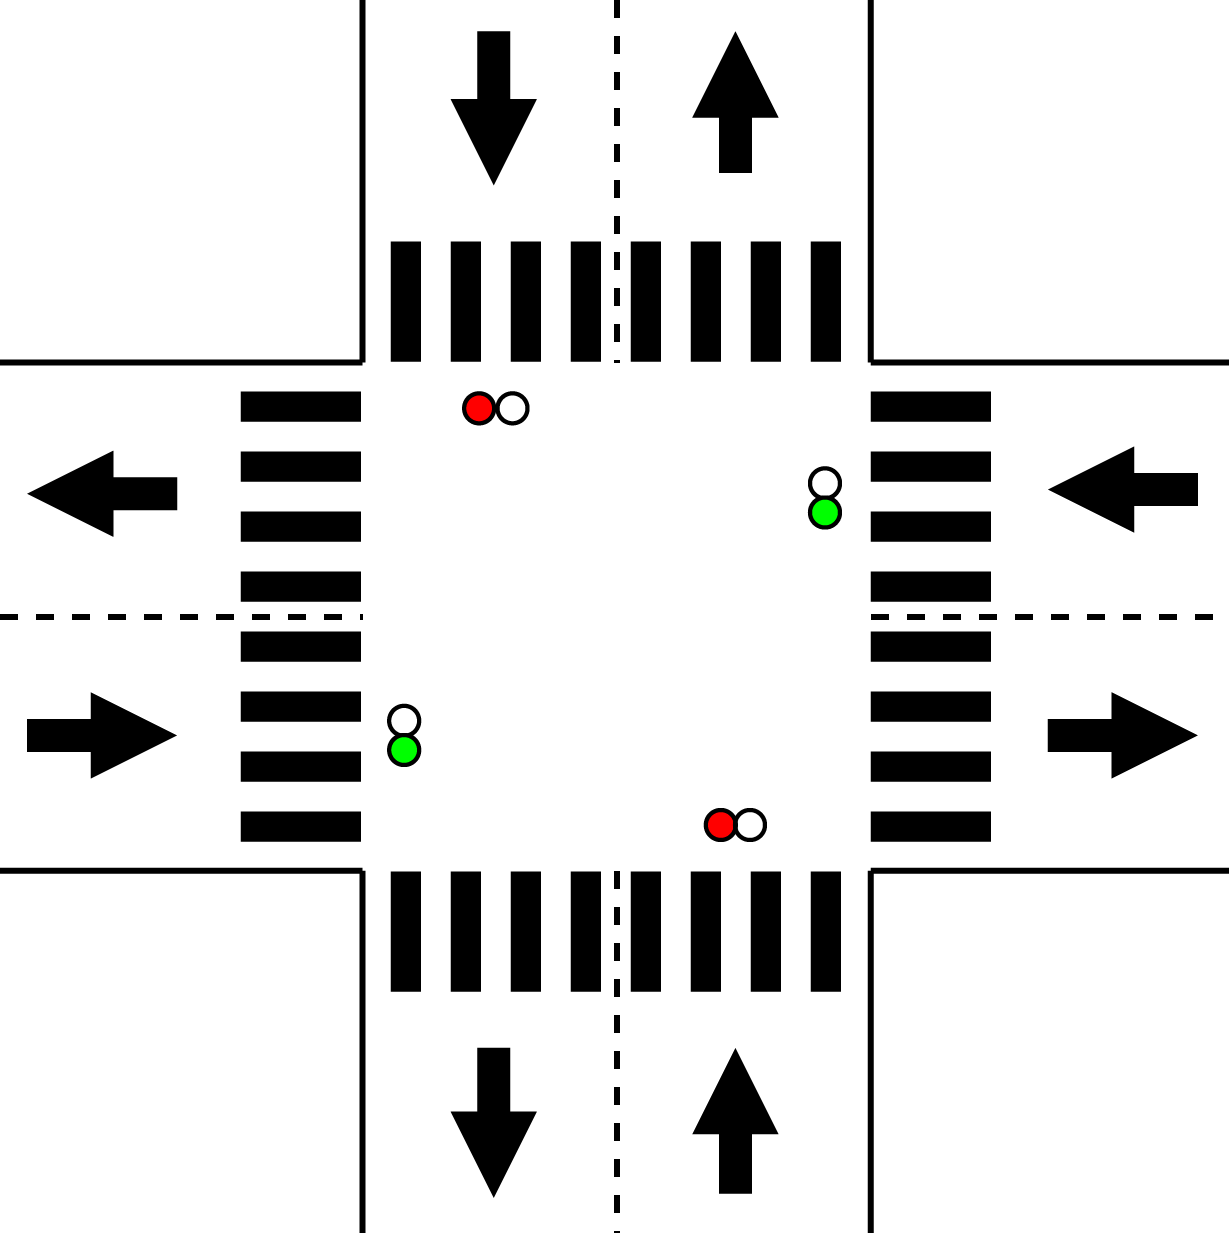
\includegraphics[width=0.5\textwidth]{picture/model/trafficlight_step1_s1.png}
    \caption{Model of the step 1}
\end{figure}

\subsubsection{Step 2: Pedestrians}
In this step, pedestrians were added and different things had to be changed to accommodate this new change. \\ 

When a pedestrians call was send by the environment, the car's traffic light that was green had to become red and the other car traffic light had to stay red. When those two traffic lights are red, the pedestrians traffic light could switch tp green. Because we also wanted fairness in our system, two assumptions were added here.
\begin{enumerate}
    \item When the pedestrians traffic light is green, we have to remember which car traffic light was previously green. This will be useful for the next assumption.
    \item We wanted fairness between the actors, even if pedestrians have the priority. The problem at the beginning was that starvation could happen if, when the pedestrians lights are green, we always switched to a specific car's traffic light. This would mean that the other car's traffic light would remain red if pedestrians are always calling. We thus added what we called a "delayed" call where, even if the pedestrians are always pressing the button, the two cars lights have to be green at least once before the pedestrians could have their lights green again. This is why the first assumption is useful, we have to remember which car's light was previously green so the cars in the other side of the crossroad don't always have to wait 2 times to be green again. \\
    As an example, if the East-West car's traffic light is green and a pedestrian pressed the button, after the pedestrians lights switch from green to red, the North-South car's traffic light is switched to green so they do not have to wait another time.
\end{enumerate}

\subsubsection{Step 3: Buses}
In this step, we added the buses generated by the environment. The idea here is that the buses have priority on the rest of the traffic. \\
When a bus is generated, the next traffic light that has to be green is the one of the bus. When the bus is crossing, all other lights are red because the bus will go through. The model can be seen as on Figure \ref{fig:step3bus}. \\

\begin{figure}[H]\label{fig:step3bus}
  \centering
    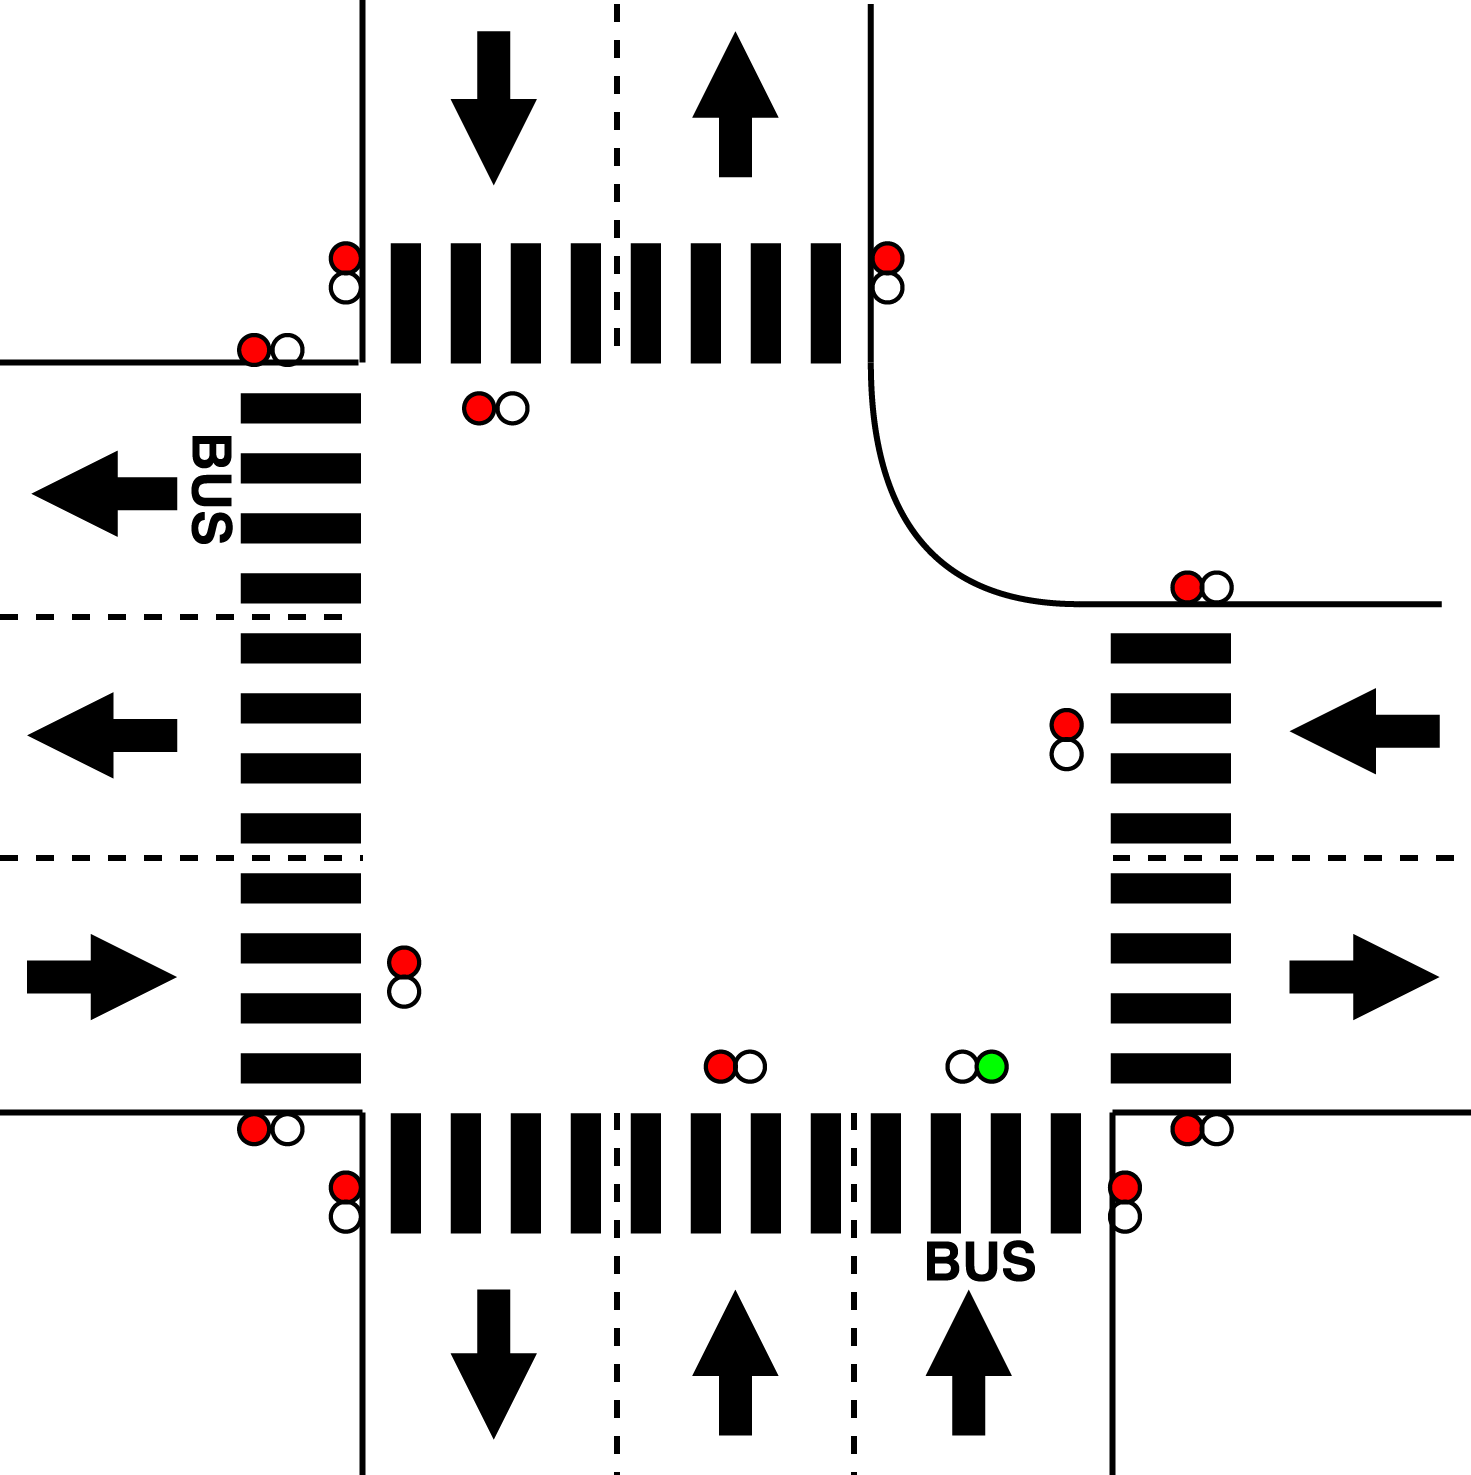
\includegraphics[width=0.5\textwidth]{picture/model/trafficlight_step3_s2.png}
    \caption{Model for the step 3}
\end{figure}


\noindent Even if the pedestrians have called to have the green lights before the bus, if a bus is generated between the call and the pedestrians green light, we will first give the green light to the bus, then the pedestrians, then the cars. This mean that the priority hierarchy is \textit{Buses-Pedestrians-Cars}.


\subsection{Uppaal Timed Automatons}
In order to formally model the system, we use several timed automatons from Uppaal. While some of those automatons are actors in the environment, the others are part of the controller.
The theory tells us that, when the environment is playing, we, humans, cannot decide the action that will be taken. For example, buses and pedestrians arrivals are unpredictable and uncontrollable, so they belong to the environment.
The actors which implement the solution for avoiding crashes belong to the controller. They interact with the environment in order to avoid crashes and thus they aim to find a winning strategy. \\
We will now give the implementations explanations of the environment and controller actors. In the first one, we will take a look at the pedestrians and buses generators while in the second one, we will look at our traffic light system that tries to find a winning situation (no crashes).

\subsubsection{Environment}
\paragraph{Crosswalk} \mbox{}\\
We will here talk about the mechanisms of our crosswalk generator done in our step 3 from Section \ref{sec:step3}. \\

\begin{figure}[H]\label{fig:crosswalk}
  \centering
    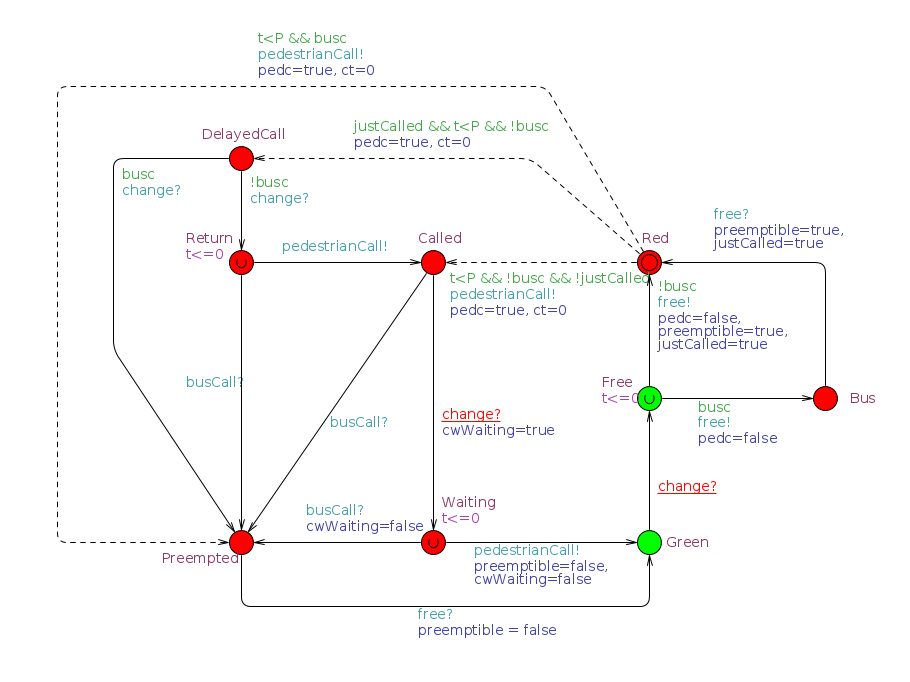
\includegraphics[width=0.9\textwidth]{picture/crosswalk.png}
    \caption{Pedestrians generator}
\end{figure}
\noindent The initial state of the pedestrians lights is Red. From this state, three different destinations states are possible:
\begin{enumerate}
  \item The Preempted state: A pedestrian call has been made but there is a bus. Since they have total priority, we will first have to wait for the bus to cross the road before we can,
  \item The DelayedCall state: If there is no bus but the pedestrians already pushed the button within a certain time period in the past, we do not give them the green light immediately to stay fair,
  \item The Called state: If a call has been made and no conditions from 1 or 2 are present, we go to this state. This state means that the pedestrian will get the green light at the end of the current timer.
\end{enumerate}
At the end, every other state will reach the Preempted one after having to wait for the end of the timer. We then switch the pedestrians lights to green. After the green state, we reach a free state because, before going back to the red state, different things can happen. Indeed, a bus could arrive and since it has the priority, we will have to give him the next green light. If no bus arrived, we go back to the red state and the basic cars traffic lights will start again. 

\paragraph{Bus} \mbox{}\\
We will here talk about the mechanisms of our bus generator done in our step 3 from Section \ref{sec:step3}. \\
As for the pedestrians, four different states can be reached. We still have Preempted, DelayedCall and Called and there meaning is the same than the ones previously defined. for the pedestrians. The only difference here is that, since the bus has priority, if the pedestrians were waiting, we first have to put the bus light to green. The rest follows the same scheme as for pedestrians lights.

\begin{figure}[H]\label{fig:bus}
  \centering
    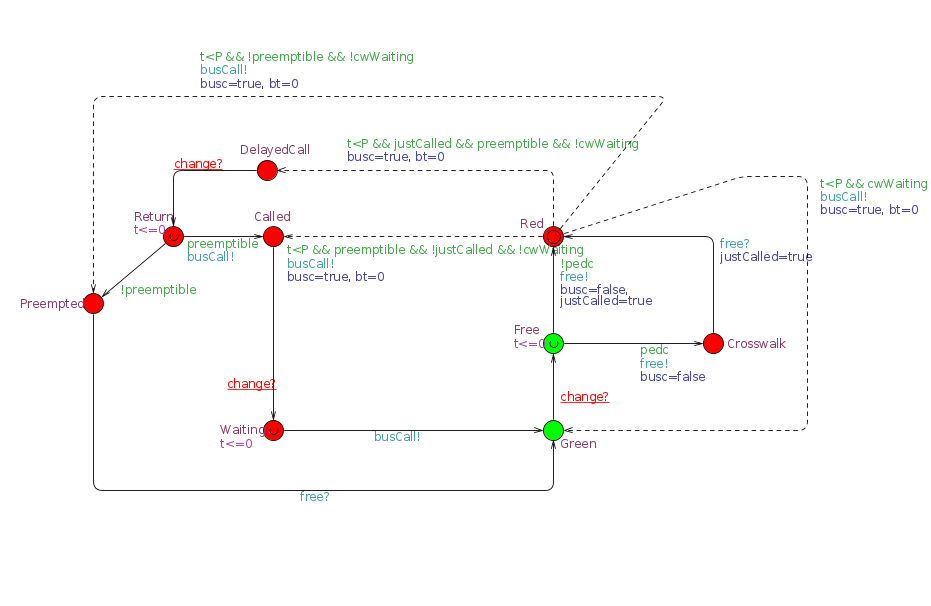
\includegraphics[width=0.9\textwidth]{picture/bus.png}
    \caption{Buses generator}
\end{figure}

\noindent Those were the two actors controlled by the environment.

\subsubsection{Controller}
\paragraph{Traffic Lights} \mbox{}\\

In this section, we will present the strategy we implemented for the controller to reach a winning strategy. \\

As said above, there are two different direction for cars traffic lights. There is the one we called Left-Right, meaning it represents the East-West lights and the Front-Back representing the North-South crossroad. Since the idea is the same, we will just explain the Left-Right one. It just has to be kwown that the initial state for the Left-Right is the red trafic light while for the other one the initial state is the green one. \\

From the red initial state, three different states can be reached:
\begin{enumerate}
  \item If a bus has been called, other traffic light has to remain red so the bus can drive through the crosswalk. We thus reach a \textit{Bus} state.
  \item If pedestrians have pushed the button, we switch to a \textit{Crosswalk} state.
  \item If no buses or pedestrians were generated and the other cars traffic lights is switching to red, we can reach a \textit{Green} state.
\end{enumerate}

